\chapter{Introduction} \label{chap:intro}

Systematic reviews are at the core of evidence-based research. They help synthesize vast amounts of literature, ensuring that decisions in science, medicine, policy, and other fields are grounded in the best available evidence. However, conducting systematic reviews is a time-intensive and often overwhelming process. Screening literature, managing citations, extracting data, limiting biases and subjectivity, and ensuring methodological rigor and replicability all demand meticulous attention to detail.

\texttt{prismAId} was created to address these challenges. It is an open-source toolkit designed to assist researchers in conducting systematic reviews more efficiently using generative AI technology.\tip{Systematic reviews require structured workflows. \texttt{prismAId} provides modular tools to help enforce best practices at each stage of the process.} By streamlining key aspects of the review process, \texttt{prismAId} helps users maintain high standards of rigor and reproducibility while reducing the manual workload.

The toolkit is designed for a diverse range of users, from researchers conducting large-scale systematic reviews to students working on literature-based projects, requiring no coding skills to operate effectively. It provides structured workflows that align with best practices in systematic reviewing, ensuring that every step -- from acquiring literature to extracting and analyzing data -- is traceable and transparent.

\bigskip

\section{The prismAId Toolkit}

A key enhancement to \texttt{prismAId} is its modular design, which now offers four specialized tools to support different stages of the systematic review process:\note{Each tool can be used independently or as part of an integrated workflow. This modular design supports diverse research needs and practices.}

\begin{itemize}
    \item \textbf{Screening Tool}: Filters manuscripts after initial search but before full-text download, using deduplication, language detection, article type classification, and topic relevance scoring to identify papers for exclusion.

    \item \textbf{Download Tool}: Acquires papers directly from Zotero collections or from URL lists, streamlining the literature acquisition phase for manuscripts that passed screening.

    \item \textbf{Convert Tool}: Transforms documents from various formats (PDF, DOCX, HTML) into plain text that can be processed by large language models.

    \item \textbf{Review Tool}: Processes systematic literature reviews based on configurable protocols, extracting structured information from scientific papers.
\end{itemize}

\begin{figure}[h]
    \centering
    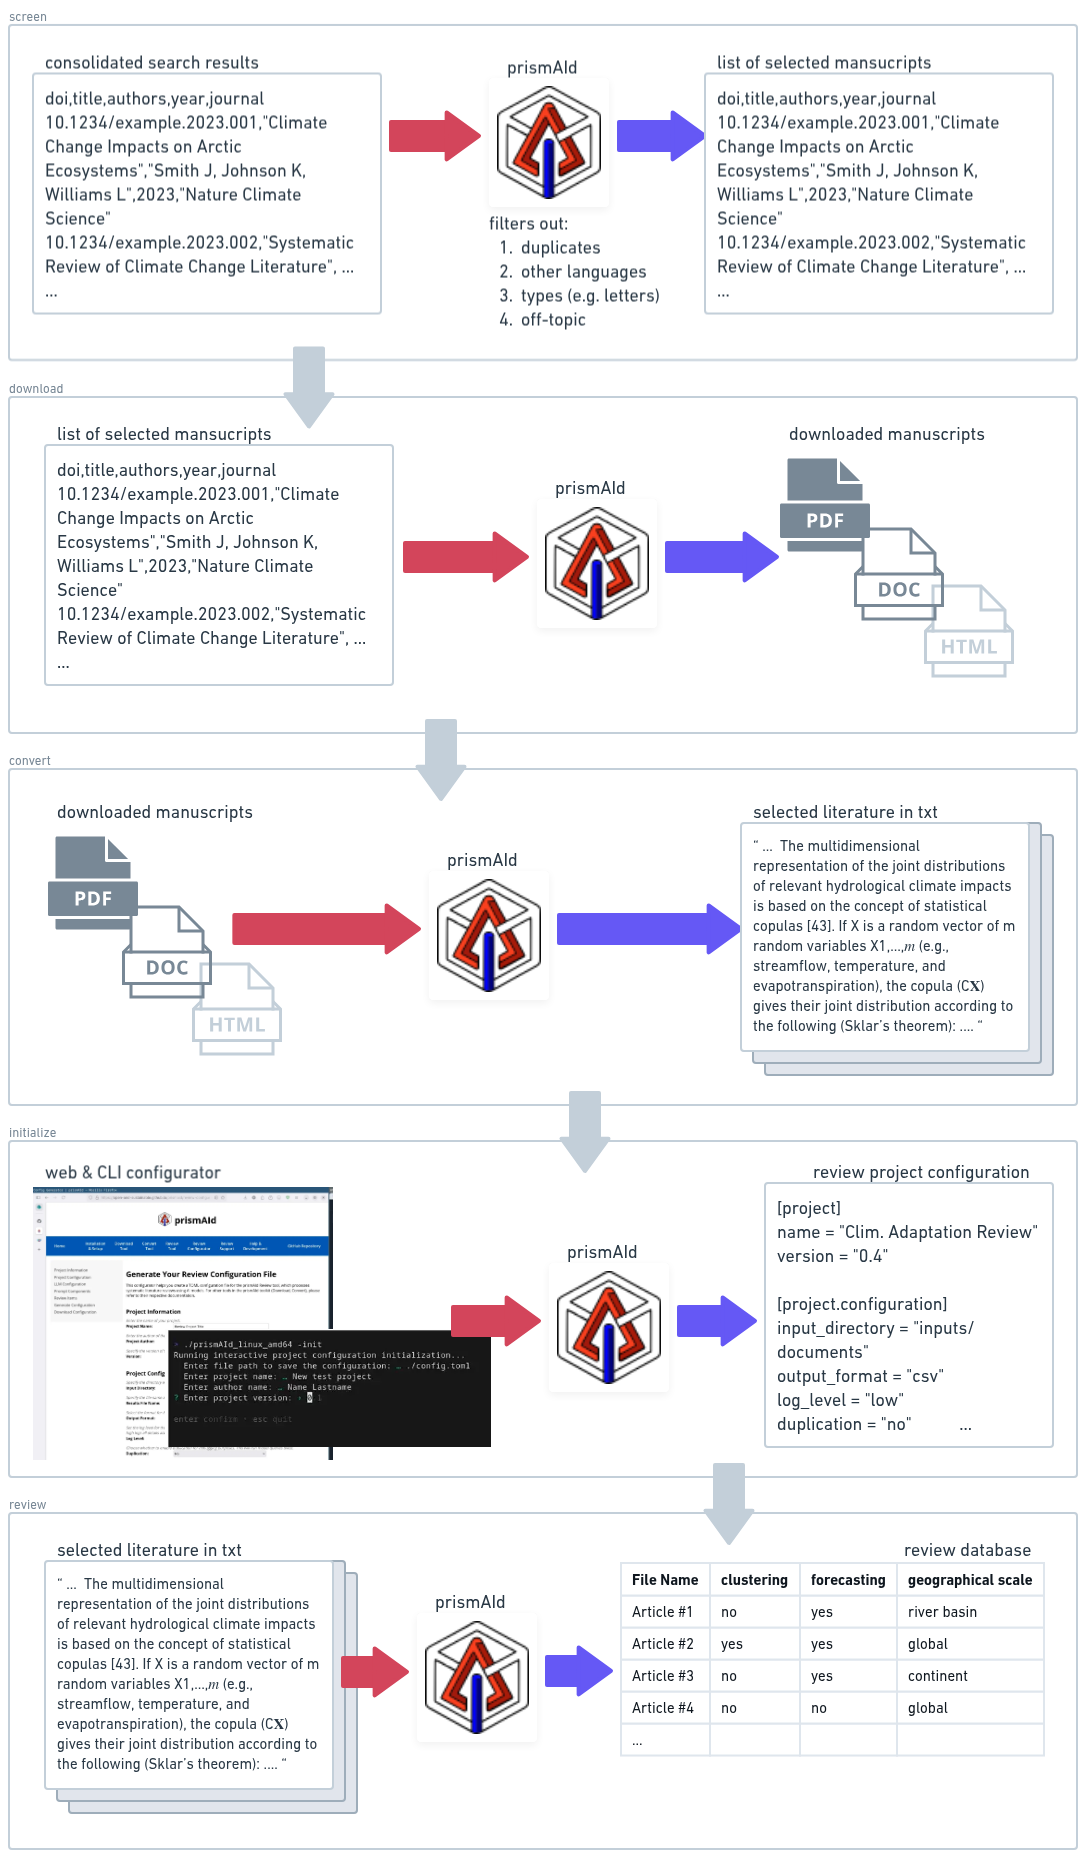
\includegraphics[width=\textwidth]{figures/prismAId_workflow.png}
    \caption{The complete prismAId workflow: from literature search through screening, downloading, conversion, to final information extraction and analysis. Each tool can be used independently or as part of an integrated systematic review pipeline.}
    \label{fig:workflow_overview}
\end{figure}

This modular approach allows researchers to integrate \texttt{prismAId} into existing workflows more flexibly, using only the components needed for their specific research context.

\section{Open Science Foundation}

One of the key motivations behind \texttt{prismAId} is its commitment to Open Science. The toolkit is fully open source, meaning its development is transparent, and researchers can inspect, modify, and contribute to its functionality. This openness ensures that systematic reviews conducted with \texttt{prismAId} can be fully reproducible and that researchers can collaborate effectively without relying on proprietary or closed software ecosystems.\warning{As an open-source toolkit, \texttt{prismAId} does not include proprietary support. Users are encouraged to engage with the community through GitHub issues or the Matrix Support Room for troubleshooting and development.}

Moreover, the open-source nature of \texttt{prismAId} allows for continuous improvement through community-driven development. Users can adapt the tools to fit their needs, extend their capabilities, and integrate them with other research software. This flexibility is particularly beneficial in a rapidly evolving scientific landscape where reproducibility and adaptability are crucial.

\section{Multi-Platform Accessibility}

\texttt{prismAId} is accessible through multiple platforms and programming languages, offering flexibility based on user preference and technical requirements:

\begin{itemize}
    \item \textbf{Standalone Binaries}: For Windows, macOS, and Linux, requiring no coding skills
    \item \textbf{Go Package}: For integration in Go-based projects
    \item \textbf{Python Package}: For integration in Python scripts and Jupyter notebooks
    \item \textbf{R Package}: For use within R and RStudio environments
    \item \textbf{Julia Package}: For integration in Julia workflows
\end{itemize}

This multi-platform approach ensures that researchers can incorporate \texttt{prismAId} into their preferred computational environments without disrupting existing workflows.

\section{Guiding Principles}

Beyond technical efficiency, \texttt{prismAId} embodies key guiding principles that impact its users:

\begin{itemize}
    \item \textbf{Transparency}: The logic behind how studies are managed and processed is open for review. There are no hidden decision-making mechanisms.

    \item \textbf{Reproducibility}: Every action taken within \texttt{prismAId} can be logged and traced, allowing others to replicate results with comprehensive documentation of methodologies.

    \item \textbf{Flexibility}: Researchers can configure \texttt{prismAId} to meet the specific requirements of their systematic review protocols and adapt it to various research domains.

    \item \textbf{Accessibility}: Easy-to-use interfaces ensure that anyone can leverage advanced AI tools for literature reviews without specialized technical knowledge.

    \item \textbf{Efficiency}: The toolkit is optimized for handling large datasets with minimal setup, reducing the time from research to results.

    \item \textbf{No Vendor Lock-in}: Users are not dependent on a single commercial provider, ensuring that research workflows remain independent.

    \item \textbf{Community and Collaboration}:\reminder{Collaboration is a core feature. Consider contributing to \texttt{prismAId} if you have ideas for improvement!} As an open-source toolkit, \texttt{prismAId} fosters collaboration among researchers, developers, and systematic review specialists.
\end{itemize}

By embracing these principles, \texttt{prismAId} is more than just a toolkit -- it is part of a broader effort to improve the accessibility, efficiency, and reliability of systematic reviews. Whether used by a lone researcher or a large team, it provides the structure and support needed to navigate complex literature and synthesize high-quality evidence using the latest advancements in artificial intelligence.

As we move through this manual,\note{This manual follows a structured approach. Refer to the \textbf{How Should You Use This Manual?} section in the Foreword for guidance on navigating the content.} you will learn how to install, configure, and effectively use each component of the \texttt{prismAId} toolkit to conduct systematic reviews. From getting started with basic setup to leveraging advanced features for more complex reviews, this guide will provide all the necessary information to integrate \texttt{prismAId} into your research workflow.
